\section*{Introduction}
This report presents the implementation and analysis of Dissipative Particle Dynamics (DPD) simulations in 2D as specified in the assignment. DPD is a mesoscopic simulation method that bridges the gap between microscopic methods like Molecular Dynamics and macroscopic methods like Computational Fluid Dynamics. In DPD, particles represent clusters of molecules rather than individual atoms, allowing for simulation of larger systems and longer time scales.
The simulation implements three types of forces between particles:
\begin{enumerate}
	\item Conservative forces (soft repulsion)
	\item Dissipative forces (friction-like)
	\item Random forces (thermal fluctuations)
\end{enumerate}
These forces combine to create a thermostat that maintains the system temperature while preserving hydrodynamic behavior.\newline
\newline
The simulation was implemented in Python, for further information regarding the implementation consult the README.md file.
\section{Test Simulation}
For the preliminary test, a system containing only fluid particles was simulated with conservative force coefficient $a_{ij} = 25$. The following checks were performed:
\begin{figure}[H]
	\begin{center}
		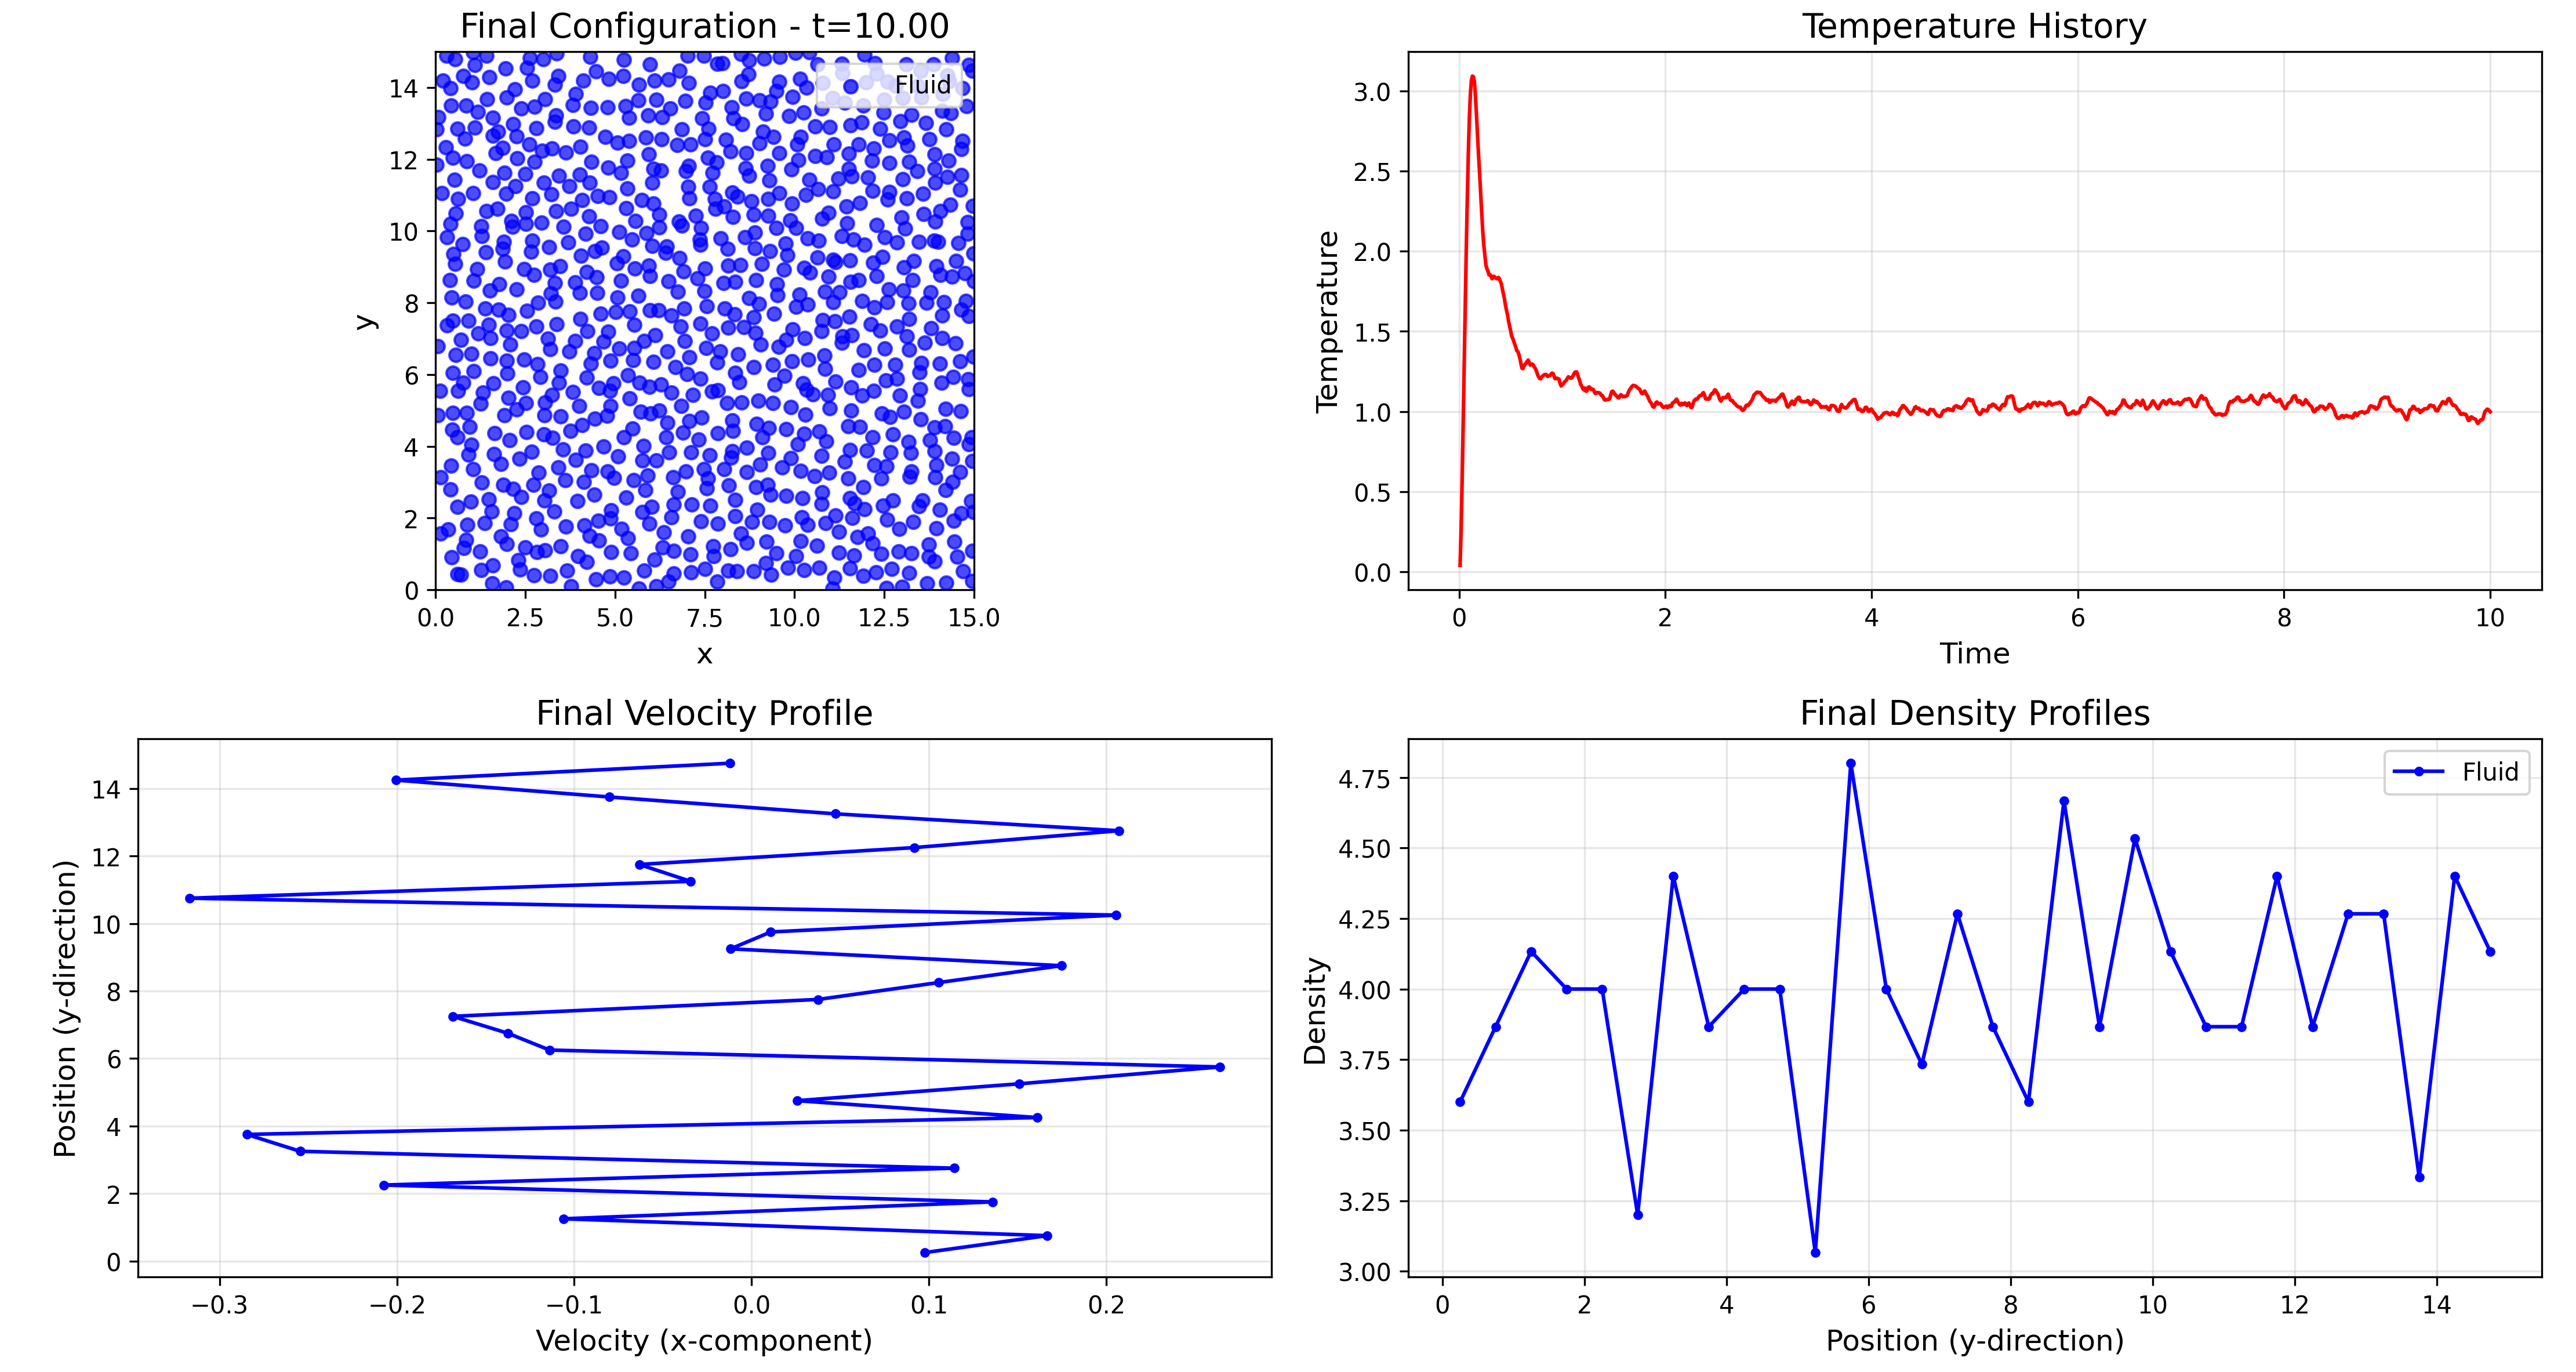
\includegraphics[width=0.95\textwidth]{figures/test_final_vis.png}
	\end{center}
	\caption{Test Scenario with $dt = 0.01$ and $1000$ steps}\label{fig:test}
\end{figure}
\subsection{Temperature Stability}
As shown in Figure \ref{fig:test}, the temperature initially spiked but quickly stabilized around $1.0$, which is the desired temperature set by the DPD thermostat parameters. This confirms proper implementation of the dissipative and random forces.
\subsection{Conservation of Momentum}
Total momentum was monitored throughout the simulation and remained conserved with only minor numerical fluctuations (not shown in figures), confirming the correct implementation of the forces.
\subsection{Timestep Dependency}
Several test runs were performed with different timestep values. For $dt = 0.01$, the system showed good stability while maintaining reasonable computational efficiency. Larger timesteps ($dt > 0.02$) led to instabilities, while smaller timesteps significantly increased computation time without substantial accuracy improvements.

